\documentclass[10pt,a4paper]{report}
\usepackage[utf8]{inputenc}  
\usepackage[T1]{fontenc}      
\usepackage[francais]{babel}
\usepackage{amsmath}
\usepackage{amsfonts}
\usepackage{amssymb}
\usepackage{graphicx}
\usepackage{hyperref}
\usepackage{caption}
\author{Thomas Citharel}
\title{Rapport de stage}
\begin{document}
	\maketitle
	\tableofcontents
	\chapter*{Introduction}
	Dans le cadre des études que j'effectue à l'\textbf{IUT d'Orléans} dans le but d'obtenir un Diplôme Universitaire de Technologie, je devais effectuer un stage d'une durée de 10 semaines afin de valider ce diplôme. Ce stage a pour but d'acquérir une première expérience professionnelle en validant les connaissances apprises durant l'année et en exercant des compétences au travers de la réalisation d'un projet.
	
	Ce stage s'est pour ma part effectué du 20 Juin au 26 Août 2016 au sein de l'association \textbf{Framasoft} dont les buts sont la promotion, la diffusion et le développement de logiciels libres, de services libres en ligne et de la culture libre.
	
	Pour ma part, j'avais pour but de développer et mettre en place une alternative à Google Calendar nommée \textbf{Framagenda}. En accord avec mon maître de stage, le choix parmi plusieurs applications existantes s'est porté sur le logiciel libre ownCloud dont la fonctionnalité principale est le service de stockage et de sauvegarde de fichiers mais qui propose de nombreuses applications tierces dont une faisant office de calendrier.
	
	\chapter{Présentation du stage}
	\section{IUT}
	L'\textbf{Institut Universitaire de Technologie d'Orléans - La Source} fait partie intégrante de l'Université d'Orléans - Tours. Il est composé de différents départements dont celui d'Informatique. Les domaines enseignés sont théoriques comme pratiques, et des enseignements complémentaires dont une langue vivante et des cours de Gestion et de communication professionnelle y sont également donnés.
	
	La formation est d'ordinaire effectuée sur la période de deux années mais l'IUT offre également aux étudiants ayant déjà un parcours dans l'enseignement supérieur la possibilité d'effectuer cette formation en une année.
	
	La formation se conclut par un stage obligatoire pour mettre en application les connaissances acquises au fil de l'année, exercer ses compétences en participant à un projet non-scolaire et idéalement en acquérir de nouvelles.
	
	\section{Présentation de la structure d'accueil}
	
	\begin{quote}
		Lorsqu'un logiciel, une œuvre ou un service est dit libre, c'est en réalité l'utilisateur final qui est libre, car il a la liberté de pouvoir lire le code source du logiciel pour comprendre comment il fonctionne, la liberté de modifier l'œuvre originale pour en faire quelque chose d'autre issu de celle-ci, et enfin d'être libre d'installer soi-même ses propres services semblables à ceux proposés en ligne.
	\end{quote}
	
	Le site internet Framasoft (pour \textbf{fra}nçais et \textbf{ma}thématiques) a été fondé en 2001 comme un site annuaire de logiciels gratuits comme ressources pour enseignants par M. Alexis Kaufmann. Quelques années plus tard, il découvre le monde des logiciels libres et devient sensible à ses valeurs en restreignant son annuaire aux logiciels uniquement libres.
	
	Le réseau Framasoft se développant, une association Loi 1901 éponyme est fondée en 2004 et acquiert le statut d'association à but non lucratif en 2008. Aujourd'hui, Framasoft est une des associations francophones les plus en pointe sur le sujet des logiciels libres (avec l'APRIL) et du respect de la vie privée (avec la Quadrature du Net). 
	
	Depuis l'annuaire de logiciels libres qui n'a cessé de se remplir, on peut également noter les projets suivants proposés par l'association :
	\begin{itemize}
		\item la \textbf{Framakey}, clé USB contenant une sélection de logiciels libres à utiliser directement sous Windows, Linux ou MacOS X ;
		\item les \textbf{Framabooks}, une collections d'ouvrages (Romans, BD, Manuels) diffusés sous différentes licences libres ;
		\item le \textbf{Framablog}, qui parle de logiciels et de culture libre en lien avec l'actualité mais propose également des traductions d'articles écrits dans des langues étrangères.
	\end{itemize}
	
	En octobre 2014, la campagne \href{https://degooglisons-internet.org/}{\textbf{\textit{Dégooglisons} Internet}} est lancée dans le but de montrer au public que des solutions (toujours libres) sont possibles face aux services proposés par les \textit{géants du net} (aussi nommés \textbf{GAFAM} pour \textbf{G}oogle, \textbf{A}mazon, \textbf{F}acebook, \textbf{A}pple et \textbf{M}icrosoft, mais il y en a plein d'autres).
	
	Depuis le lancement de la campagne Framasoft a déjà ouvert une vingtaine de services en ligne et il en est prévu davantage d'ici la fin de la campagne en 2018.
	
	Framasoft utilise donc des applications web libres existantes ou développe ses propres alternatives pour proposer à des personnes non-techniques des services viables.
	
	Ainsi, l'association a fait développer des solutions spécialement pour proposer \textbf{Framapic} (hébergement d'images : alternative à Imgur, Flickr), \textbf{Framalink} (raccourcisseur d'url : alternative à bit.ly) et \textbf{Framadrop} (service de transfert de fichiers : alternative à WeTransfer).
	
	Il est important de remarquer que Framasoft n'ambitionne pas de devenir le prochain géant du web. L'association reste à but non lucratif et a de plus une volonté de décentraliser ses activités au sein de structures locales qui seraient des « hébergeurs de services de proximité ».
	
	L'association ayant comme but de sensibiliser le grand public aux valeurs du logiciel libre, elle est très souvent invitée à s'exprimer lors de manifestations du genre, comme j'ai pu participer à Nevers le week-end du 24 au 26 Juin.
	
	\subsection{Quelques chiffres}
	Framasoft compte aujourd'hui cinq salariés ainsi que deux stagiaires, ainsi qu'une vingtaine de membres actifs. Côté services, on compte aujourd'hui xxx visites par mois sur le Framablog, un sondage créé toutes les xx secondes sur Framadate et xxx pads sur Framapads. Les livres édités par Framasoft sont au nombre de xx, et leur ventes totales avoisine les xx. Enfin, grâce à l'éclatement géographique de ses membres, Framasoft est présent sur la quasi-totalité des événements liés au logiciel libre en francophonie.
	
	\section{Présentation du projet}
	
	\subsection{ownCloud}
	\textbf{ownCloud} est une application web libre écrite dans le langage de programmation PHP. Elle a été initialement créée en 2008 comme une alternative au service Dropbox par Frank <Inserer nom Allemand ici>.
	
	Elle consiste en un cœur (dénommé par la suite comme le \textit{core}) qui s'occupe essentiellement de la gestion des utilisateurs, de la gestion des fichiers, de la gestion des partages et de la fédération et propose des API aux applications tierces. D'autres applications (comme une application de gestion de calendrier, de gestion de contacts, de client de messagerie électronique, de prise de notes ou encore de lecteur de flux RSS) peuvent ainsi intégrées à ownCloud.
	
	ownCloud peut être installé sur tout hébergement mutualisé qui propose au moins une version de PHP supérieure ou égale à la version 5.4, et propose également des paquets installables automatiquement sur les principales distributions à travers leurs dépôts. De plus, il est proposé à l'administrateur le choix en termes de système de bases de données entre \textit{SQLite}, \textit{MariaDB}/\textit{MySQL} et \textit{PostgreSQL}.
	
	Quelques mois avant que mon stage débute, ownCloud a sorti une version 9 qui a transféré le module DAV (serveur responsable du calendrier et des contacts) dans le \textit{core} et la logique de l'application Calendar a été refaite complètement quasiment intégralement en JavaScript à l'aide du framework \textit{AngularJS}.
	
	D'autre part, la communauté et l'entreprise derrière ownCloud se sont pris le chignon, aboutissant à la création d'un \textit{fork} du nom de NextCloud. Heureusement, je me suis aperçu que les deux projets continuaient à communiquer et à échanger du code.
	
	\subsection{Les standards de gestion de calendrier}
	Un serveur de calendrier doit suivre les standards \textbf{CalDAV}, qui est une extension du protocole \textbf{WebDAV} appliquée aux fichiers \textbf{iCalendar} (\textit{.ics}). WebDAV est un protocole de gestion de fichiers sur serveurs distants conçu comme une extension du standard HTTP. Il a commencé par être standardisé par l'IETF en xxxx.
	
	\href{https://tools.ietf.org/html/rfc2445}{iCalendar}, pour sa part est un standard assez vieux (1998 !) qui décrit le format d'un fichier agenda. Ce format est beaucoup décrié aujourd'hui car étant assez lourd et complexe à manipuler. Heureusement, il existe de nombreuses librairies nous évitant de traiter directement ce format.
	
	Dans notre cas, le serveur est - heureusement - géré avec le concours d'une librairie du nom de \textbf{SabreDAV} qui prend en charge CalDAV, CardDAV (pour les contacts) et WebDAV. Cette librairie fonctionne avec un système de plugins nous permettant de l'adapter pour notre utilisation dans ownCloud.
	
	Il est important de remarquer que si les protocoles et standards internet pour la gestion de calendrier sont définis et correctement documentés, leur implémentations dans les applications clientes ou serveur sont plus qu'hasardeuses et la liste des fonctionnalités supportées peut être assez différente d'une application à l'autre.
		
	Ainsi, c'est la société Apple qui est à la pointe des derniers standards dans son application \textit{iCal} (désormais nommée plus simplement \textit{Calendar}). N'ayant pas de machine Apple, je n'ai pu profiter de ce logiciel pour mes tests.
	
	Le standard WebDAV décrit un protocole pour gérer des ressources - dans notre cas des calendriers - comme un ensemble de méthodes qui étendent celles définies par le standard HTTP. Ces méthodes sont utilisées par des requêtes et des réponses qui structurent les données à l'aide du format XML. Par exemple pour récuperer les propriétés d'une ressource on va utiliser la méthode PROPFIND et si on veut modifier les propriétés d'une ressource la méthode PROPPATCH.
	
	<Image d'exemple d'une requête avec du XML dedans>
	
	Le standard WebDAV décrit également ce que sont les collections de ressources et comment les droits d'accès (nommés ACL) sont gérés. Par exemple, un utilisateur ne peut accéder qu'à ses fichiers ou à ceux que d'autres utilisateurs ont partagés avec lui.
	
	Le standard XML définit les balises appartenant à un espace de noms. En l'occurence nous avons des balises représentant les propriétés de notre ressource, elle appartiennent ainsi à autant des espaces de noms différents qu'il existe de standards différents qui s'appliquent (IETF, DAV, CalendarServer c'est à dire Apple, et ownCloud pour nos propres propriétés).
	
	\subsection{Buts du stage}
	L'application Framagenda réalisée comme une alternative à Google Agenda se basant sur une application de calendrier existante devait essayer d'avoir un nombre de fonctionnalités équivalent ainsi qu'une apparence moderne et utilisable par le grand public.
	
	Ainsi, des applications plus anciennes qui possédaient des fonctionnalités plus avancées ont été écartées car l'interface était non intuitive et la mauvaise qualité du code signifiait apporter une dette technique assez significative.
	
	L'application Calendrier d'ownCloud permettait déjà les fonctionnalités essentielles suivantes :
	\begin{itemize}
		\item Créer et supprimer des calendriers auquels sont associés un nom et une couleur et éditer ces propriétés. Les afficher ou bien les masquer ;
		\item Créer des événements, les supprimer ou les éditer. Quelques propriétés liées à un événement sont ses dates de début et de fin, sa localisation et évidemment sa dénommination. On trouve aussi des fonctionnalités plus avancées, comme pouvoir préciser les participants, pouvoir définir différentes occurences de ce même événement, etc ;
		\item Voir le calendrier sous forme d'un jour ou d'une semaine (comme un agenda), ou bien tout le mois en entier ;
		\item Partager un calendrier (en lecture seule ou en écriture) avec une personne ou un groupe de personnes ;
		\item Importer des événements d'un fichier .ics dans un calendrier.
	\end{itemize}
	
	A ces fonctionnalités déjà présentes j'ai dû ajouter les fonctionnalités suivantes :
	
	\subsubsection{Permettre de rendre un calendrier public et l'afficher publiquement}
	
	\begin{figure}[ht]
		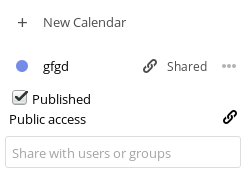
\includegraphics[width=0.25\paperwidth]{images/fonctionnalitepublie.png}
		\label{normal_case}
	\end{figure}
	
	La première tâche était la mission principale. Elle est liée premièrement à l'implémentation du protocole de publication d'un calendrier tel que défini par Apple à travers un plugin spécialisé dans le cœur d'ownCloud. D'autre part, il nous faut également une interface utilisateur dans l'application Calendrier qui permette de publier et dé-publier un calendrier. Enfin, il était nécessaire de proposer une vue « publique » accessible à tous sans être enregistré pour les calendriers publiés.

	\begin{figure}[ht]
		\centering
		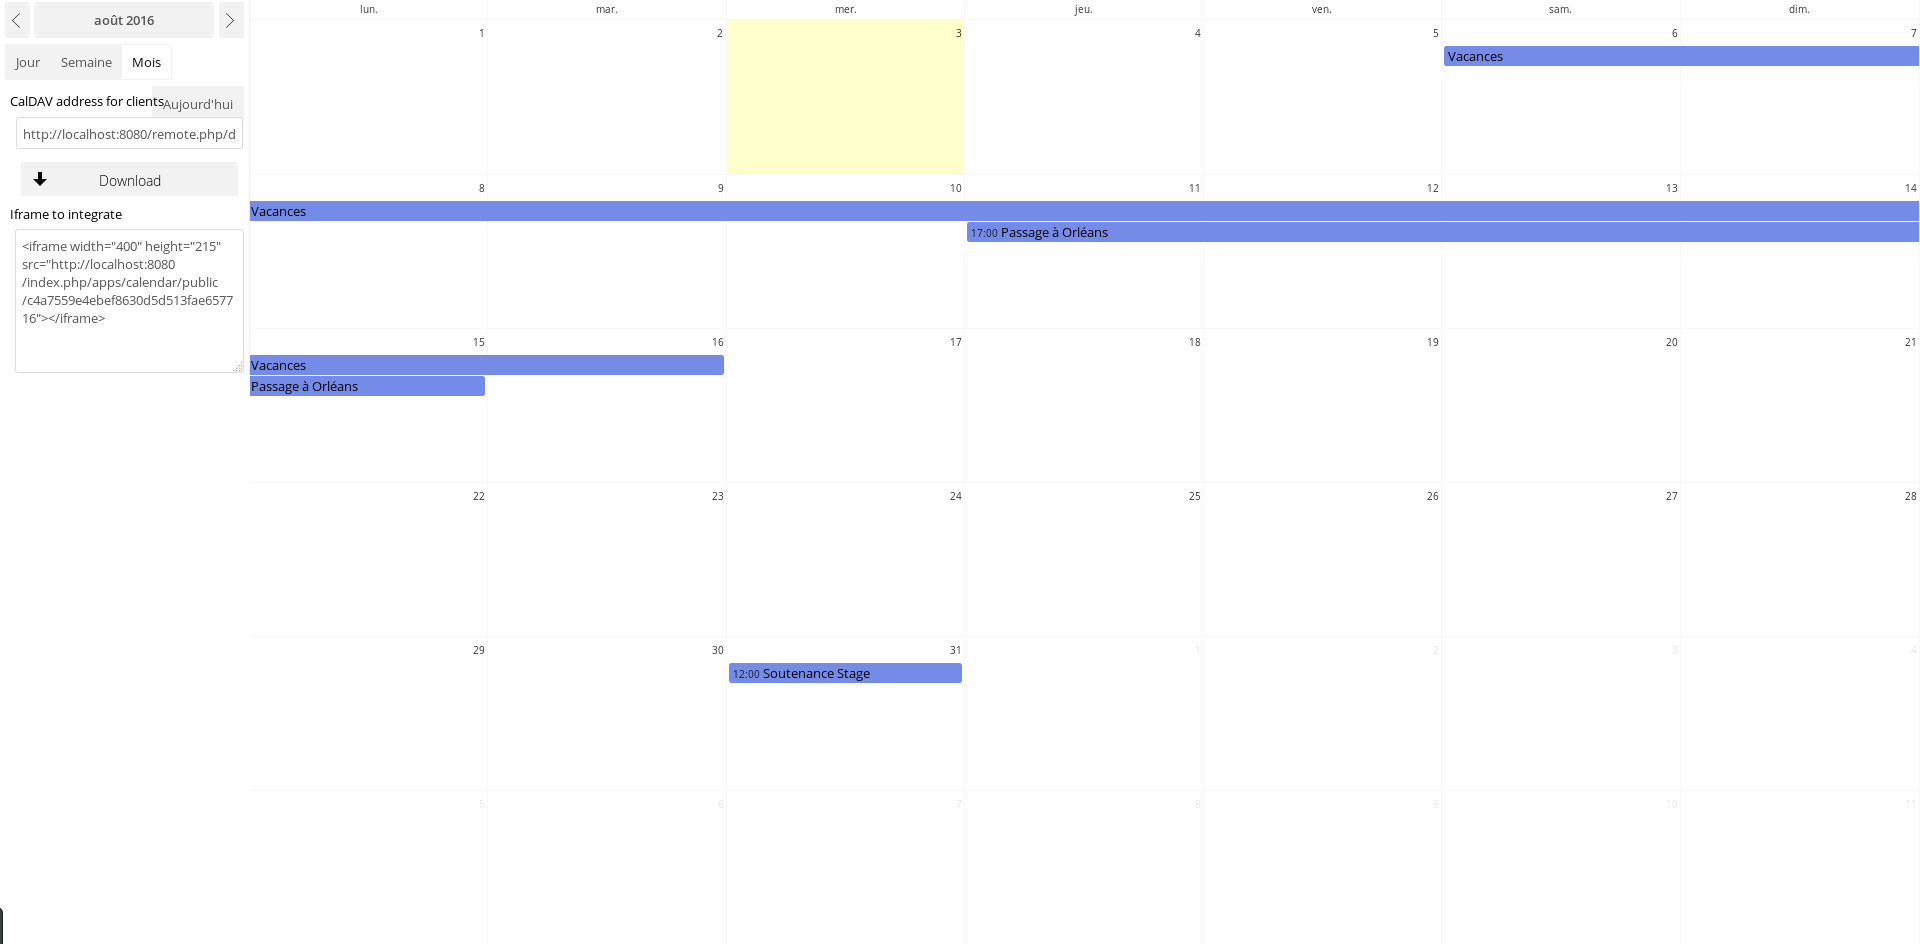
\includegraphics[width=1.25\textwidth]{images/calendrier-vue-publique.png}
		\caption*{Vue publique d'un calendrier}
		\label{normal_case}
	\end{figure}

	
	\subsubsection{Permettre d'afficher ce calendrier public sur des pages web externes}La seconde tâche était assez simple et consistait surtout à configurer l'application correctement pour autoriser l'intégration à l'intérieur de sites tiers, et de rendre son apparence acceptable.
	
	\begin{figure}[ht]
		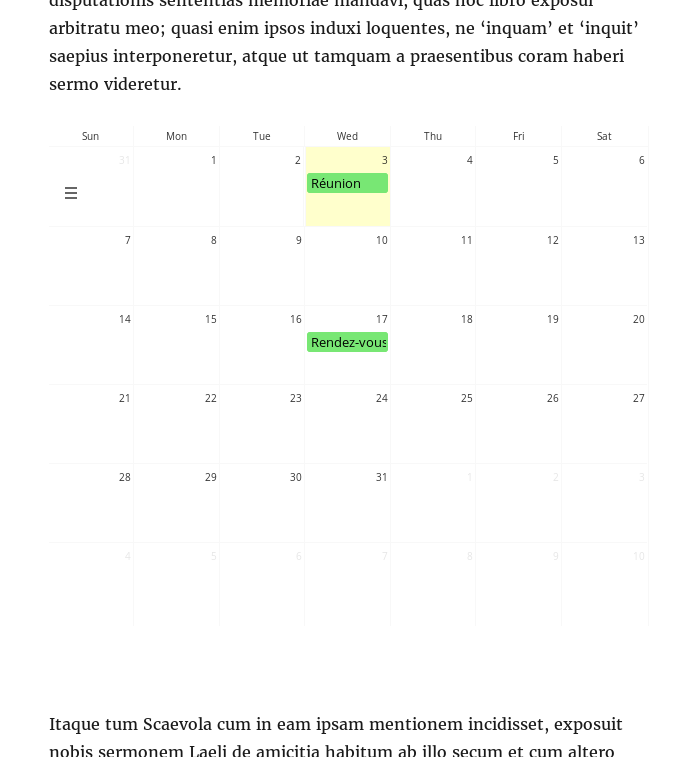
\includegraphics[width=0.5\paperwidth]{images/integration_wordpress}
		\caption*{Intégration d'un calendrier public dans une page Wordpress}
		\label{normal_case}
	\end{figure}
	
	\subsubsection{Permettre de s'abonner à des calendriers}
	
	\begin{figure}[ht]
		\centering
		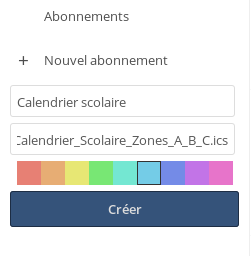
\includegraphics[width=0.30\textwidth]{images/creation_abonnement.png}
		\caption*{Formulaire pour ajouter un calendrier public}
		\label{normal_case}
	\end{figure}
	
	La troisième tâche consistait à pourvoir une fonctionnalité d'abonnement à des calendriers issus d'une source publique sur internet dans l'application Calendrier d'ownCloud. En effet, l'implémentation des abonnements selon le standard CalDAV était déjà réalisée dans le cœur d'ownCloud, il suffisait de réaliser les bons appels aux API et de gérer les fichiers distants du côté de l'application Calendrier.
	
	\section{Environnement technique}
	J'ai d'abord effectué mon développement à l'aide de l'éditeur \textit{Atom}, mais je lui ai vite préféré l'autocomplétion plus intelligente de l'éditeur \textit{phpStorm}. ownCloud utilise git pour la gestion de leur code à travers la forge logicielle \textit{Github}, qu'ils utilisent également pour le système de tickets. Je me suis donc abonné par courrier électronique à certaines discussions dès le départ afin de suivre certains travaux en cours.
	
	Pour ce qui est de Framagenda, j'ai d'abord eu accès à une machine virtuelle afin d'effectuer des tests ne pouvant être effectués sur ma machine locale, comme l'envoi de courriers électroniques à partir d'un serveur. D'autre part, une instance sur internet m'a aussi permis de demander à des personnes au sein de l'association de faire des tests fonctionnels et d'avoir des premiers retours.
	
	Lors de la mise en production, une machine virtuelle a été dédiée à Framagenda, et l'administrateur système s'est occupé de la configuration de sécurité de base et de la mise en place d'un certificat \textsc{HTTPS} avec le projet \textit{Let's Encrypt}, tandis que j'ai mis en place l'application en elle-même ainsi que configuré proprement le serveur web \textit{nginx} et le serveur de base de données \textit{MariaDB}.
	
	Le code de l'application installé sur les machines provenait directement de mon propre dépôt git sur la forge logicielle proposée par l'association - Framagit - et dont le code correspondait à peu près à celui proposé sur Github, les modifications particulières applicables pour Framagenda en plus. Enfin, là où j'avais une branche pour chaque fonctionnalité dans Github, je m'efforçais d'avoir une branche « produit fini » où les différentes branches étaient fusionnées dans Framagit.
	
	\chapter{Whatever}
	\section{Historic}
	La première semaine de mon stage a été dédiée à l'étude du fonctionnement du cœur d'ownCloud et de son intégration avec la librairie SabreDAV. J'ai dû également rechercher beaucoup d'informations sur les standards de CalDAV (ainsi que ce qui n'est pas standardisé !) car la synchronisation devait fonctionner à partir des clients existants.
	
	D'autre part, j'ai également dû lire beaucoup du code de l'application Calendrier, car elle est développée à l'aide du Framework AngularJS qui n'est pas exactement une technologie que je maîtrisais.
	
	<Schema du fonctionnement du bouzin>
	
	SabreDAV (coeur, plugins)
	ownCloud - dav (classes qui étendent le coeur, plugin chargés à la demande : certains de SabreDAV, certains à nous)
	
	\section{Publication}
	Pour pouvoir publier un calendrier il nous fallait donc plusieurs choses : d'abord introduire dans le \textit{core} la gestion de cette propriété, c'est à dire lorsqu'on interroge la ressource calendrier sur ses propriétés, fournir celle-ci en disant le cas échéant si le calendrier est publié.
	Ensuite, il nous fallait introduire un mécanisme pour pouvoir répondre à un appel d'API pour publier ou dépublier le calendrier. Enfin, il fallait que le calendrier publié soit mis dans une collection de ressources à part accessibles à tout le monde.
	
	Je n'ai pas compris cet aspect tout de suite. Je pensais qu'il suffisait de garder la ressource existante et de forcer l'authentification à être désactivée dans ce cas précis.
	
	Tous ces mécanismes ont été réalisés de la même manière (avec les mêmes noms de propriétés) selon laquelle Apple utilise la fonctionnalité de publication dans son application Calendar, et le serveur de Calendrier ownCloud devrait donc être compatible avec ce client.
	
	Il a d'abord fallu changer un peu le \textit{backend}, c'est à dire la manière dont l'application va traiter les données pour les stocker dans la base de donner pour sauvegarder ce nouveau statut du calendrier.
	
	J'ai profité du fait que les partages de calendrier entre utilisateurs étaient stockés dans une table \textit{dav\_shares} où la colonne \textit{access} comprenait un chiffre qui désignait le niveau d'accès au fichier.
	
	J'ai donc rajouté un niveau d'accès qui correspondait à un partage public, ainsi qu'une nouvelle colonne pour stocker l'URL une fois qu'elle serait publiée. 
	
	En effet, l'URL publique se consitue ainsi : 
	\begin{verbatim}
	https://mondomaine.tld/index.php/apps/calendar/public-calendar/<token>
	\end{verbatim}
	qui va chercher les données du calendrier à l'adresse
	\begin{verbatim}
	https://mondomaine.tld/remote.php/public-calendars/<token>
	\end{verbatim}
	
	Comme le token est calculé à partir des paramètres du calendrier, si je n'avais pas cette colonne supplémentaire pour stocker l'adresse finale de la ressource, il faudrait itérer sur tous les calendriers partagés sur le serveur et vérifier que leur hash correspond bien à celui fourni dans l'URL publique. Alors que dans ce cas je peux savoir directement s'il existe un calendrier pour cette URL publique et le cas échéant récupérer ses informations.
	
	Ensuite, il a fallu écrire un plugin pour SabreDAV pour générer ces propriétés proprement et l'intégrer dans le serveur. Une classe s'occupant de la sérialisation - c'est à dire la conversion des données dans un format texte structuré, ici XML - a également été nécessaire.
	
	On notera que la propriété transmise - l'url du calendrier publié - est connue dès la création du calendrier (car basée sur un \textit{hash} de son identifiant et d'un sel) et est transmise par la propriété \textit{pre-publish-url} avant la publication et ensuite par la propriété \textit{publish-url} dès lors que le calendrier est publié.
	
	Pour prendre en charge la publication et la dépublication, notre plugin a dû intercepter les requêtes POST qui contenaient une propriété particulière.
	En l'occurence, si la requête s'effectuait à l'adresse d'une ressource calendrier et qu'elle contenait l'élément XML \textit{publish-calendar} ou \textit{unpublish-calendar}, nous traitons la requête dans un sens ou dans l'autre et empêchons le traitement de cette dernière par d'autres plugins.
	
	Enfin, pour qu'un calendrier soit disponible publiquement, il a fallu créer un type spécifique de collection de ressources sur lesquelles un utilisateur non-authentifié peut lire les ressources.
	
	De ce côté le serveur \textit{core} était prêt. Dans l'application Calendrier il fallait proposer une extension de l'interface pour permettre à l'utilisateur possédant un calendrier de pouvoir le publier et le dépublier. Ensuite, il fallait fournir à l'utilisateur le lien de l'interface web publique, qui lui fournir également d'autres informations comme les adresses de synchronisation (CalDAV) ou le lien de téléchargement du fichier calendrier \textit{.ics}.
	
	Cette interface web publique devait par nature se passer d'authentification, et également ne pas montrer l'intégration de l'application au système ownCloud, ne montrant que le calendrier et des informations sur celui-ci.
	
	J'ai cherché un moment comment contourner l'intégration à ownCloud avant de me rendre compte à l'aide du code d'autres applications existantes qu'il s'agissait d'un simple paramètre à passer au \textit{template}, hélas non documenté.
	
	Les détails d'un événement qui sont normalement éditables pour le possesseur du calendrier seraient ici uniquement en lecture-seule.
	
	Enfin, une fonctionnalité que j'ai ajoutée plus tard dans le développement est l'envoi de messages électroniques lorsque le calendrier est publié pour notifier des personnes de sa publication.
	
	\section{Les abonnements}
	Le standard CalDAV prévoit la possibilité de s'abonner (ou souscrire) à des sources de calendriers externes (publiques sur internet). Cette fonctionnalité était déjà implémentée dans le \textit{core}, mais l'interface de l'application Calendrier ne permettait pas de le faire. 
	
	J'ai donc rajouté cette fonctionnalité en étendant le modèle AngularJS correspondant à un calendrier pour en faire un modèle d'un abonnement, et rajouté dans l'interface une zone pour ajouter une nouvelle souscription. 
	
	Afin de ne pas récuperer à chaque fois le calendrier distant en ligne, un système de proxy met en cache le fichier calendrier distant.
	
	\section{Les tests unitaires}
	Les tests unitaires n'étaient pas forcément requis dans le cas de mon développement, mais ils étaient obligatoires dans le cas où je voulais remonter le code \textit{upstream} (en amont) à la communauté. ownCloud, NextCloud et la plupart des applications développent en utilisant la technique d'intégration continue, c'est-à-dire que chaque nouveau morceau de code apporté sur Github lançait l'exécution de la batterie de tests au complet. 
	
	Chaque nouvelle méthode de mon code devait par conséquent s'accompagner d'un test qui devait être préalablement vérifié en local. Si une partie du code que j'avait apportée n'était pas testée, alors le \textit{code coverage}, la proportion de code couvert par les tests par rapport au code complet baissait et cela m'était automatiquement signalé. Les tests unitaires étaient réalisés à l'aide du \textit{framework} de test \textit{PHPUnit} pour le code PHP et de la librairie \textit{Karma} pour le JavaScript de l'application Calendrier.
	
	\section{Les trucs annexes}
	Mon stage consistait avant tout à implémenter de nouvelles fonctionnalités dans l'application Calendrier existante, mais il fallait également que celle-ci soit prête à être utilisée dans Framagenda sans \textit{bugs} flagrants. Ainsi, j'ai corrigé quelques problèmes tiers dans le \textit{core} ou l'application Calendrier.
	On peut citer par exemple les propriétés CalDAV d'un abonnement à un calendrier qui n'étaient pas proprement sauvegardées lors d'une requête de mise à jour ou encore les événements d'un calendrier qui s'effaçaient si jamais l'éditeur était ouvert puis l'action d'édition annulée. 
	
	De plus, afin d'avoir un style de code commun pour tous les contributeurs dans les feuilles de style CSS de l'application Calendrier, j'ai proposé d'utiliser un outil de \textit{lint} CSS et corrigé toutes les feuilles de style en accord. 
	
	Cet outil signale lorsque le code écrit ne suit pas les règles définies, par exemple l'espacement entre les blocs CSS ou l'écriture de règles désuètes.
	
	J'ai aussi ajouté les vérifications faites par cet outil au système d'intégration continue de sorte que si quelqu'un propose une \textit{pull request} qui ne satisfasse pas les règles, elle soit marquée comme erronée.
\end{document}